\section{Higher-Order Regression}
\subsection{Distribution of $B$: }
Let us suppose we are trying to fit the dataset to a functional equation of the form:
\[
    Y = \beta_0 + \beta_1 x + \beta_2 x^2 + \cdots + \beta_m x^m + \epsilon
\]
where $\epsilon \sim \mathcal{N}(0, \sigma^2)$.
We have to find the value of $B$ (the estimator of $(\beta_0, \beta_1, \cdots, \beta_m)$) that minimizes
\[
    \sum_{i=1}^n (Y_i - B_0 - B_1 x_i - B_2 x_i^2 - \cdots - B_m x_i^m)^2
\]  
Taking the derivative w.r.t each of the $B_i's$, we get 
\begin{align*}
    &\sum_{i=1}^{n} Y_i = nB_0 + B_1 \sum_{i=1}^{n} x_i + B_2 \sum_{i=1}^{n} x_i^2 + \cdots + B_m \sum_{i=1}^{n} x_i^m\\
    &\sum_{i=1}^{n} x_i\cdot Y_i = B_0 \sum_{i=1}^{n} x_i + B_1 \sum_{i=1}^{n} x_i^2 + B_2 \sum_{i=1}^{n} x_i^3 + \cdots + B_m \sum_{i=1}^{n} x_i^{m+1}\\
    &\cdots\\
    &\sum_{i=1}^{n} x_i^m\cdot Y_i = B_0 \sum_{i=1}^{n} x_i^m + B_1 \sum_{i=1}^{n} x_i^{m+1} + B_2 \sum_{i=1}^{n} x_i^{m+2} + \cdots + B_m \sum_{i=1}^{n} x_i^{2m}
\end{align*}
Let us suppose that the matrix $X$ is defined as $X_{ij}=x_i^j$. Note that $A=X^T\cdot X$ is a matrix that satisfies $A_{ij}=\sum_{k=1}^n x_k^{i+j}$ where $A_{ij}$ is the element in the $i\textsuperscript{th}$ row and $j\textsuperscript{th}$ column of $A$. Let $Y$ be the vector of $Y_i$'s. Then, the above equations can be written as:
\[
    X^T\cdot Y = (X^T\cdot X)\cdot B
\]
We claim that $X^T \cdot X$ is invertible as long as all values of $x$ are distinct. To prove this, we first prove $X$ is invertible. If that is the case, then $X^T$, which has the same determinant as $X$, is invertible, and their product also has a non-zero determinant and is invertible. For the proof of the claim that $X$ is invertible, let us assume for the sake of contradiction that the columns of this matrix are not linearly independent.\\
That is, let us assume $c_0 v_0 + c_1 v_1 + \cdots + c_m v_m = 0$ where the $c_i$'s are the columns of X and $v_i$'s are real numbers, not all zero. Then we get on the $k\textsubscript{th}$ coordinate (for $k \in \{1,\cdots n\}$):
\[
    v_0 + v_1 x_k + \cdots + v_m x_k^m = 0
\]
which means $x_k$ is a root of the polynomial $v_0 + v_1 x + \cdots + v_m x^m$. Since this polynomial has at most $m$ roots, we get that two of the $x_k$'s must be equal, which contradicts our assumption that all $x$'s are distinct.\\
Hence, $X^T \cdot X$ is invertible, and we get that $B$ is given by:
\[
    B = (X^T\cdot X)^{-1}\cdot X^T\cdot Y
\]
Thus, $B = C\cdot Y$ for some matrix $C$, with m rows and n columns.\\
$B_{i-1} = \sum_{j=1}^{n} C_{ij} Y_j$ is a linear combination of Gaussian random variables, and hence is Gaussian.\\
$B$ is a (m+1)-tuple of Gaussian random variables.
\subsection{Mean and Standard Deviation of $B$: }
We know $Y=\beta X+\epsilon$, where $\beta=(\beta_0, \beta_1, \cdots, \beta_m)$ and $\epsilon \sim \mathcal{N}(0, \sigma^2)$.\\
\begin{align*}
    E[B] &= E[(X^T\cdot X)^{-1}\cdot X^T\cdot Y]\\
    &= (X^T\cdot X)^{-1}\cdot X^T\cdot E[Y]\\
    &= (X^T\cdot X)^{-1}\cdot X^T\cdot \beta X\\
    &= (X^T\cdot X)^{-1}\cdot X^T\cdot X\cdot \beta \\
    &= \beta
\end{align*}

Above, notice that we have used the fact that the component-wise computation of the mean of B can be done simultaneously.

To find the variance, we again use matrix $C$ as defined above. $B_{i-1}=\sum_{k=1}^{n} C_{ik} Y_k$ and $B_{j-1}=\sum_{k=1}^n C_{jk} Y_k$.\\
Hence, Cov$(B_{i-1}, B_{j-1})$ = Cov$(\sum_{k=1}^{n} C_{ik} Y_k, \sum_{k=1}^{n} C_{jk} Y_k)$ = $\sum_{r=1}^n \sum_{l=1}^n C_{il} C_{jr} \text{Cov}(Y_l, Y_r)$.\\
Now, $Y_l$ and $Y_r$ are independent for $l \neq r$, and hence Cov$(Y_l, Y_r)=0$ for $l \neq r$ and Var($Y_l$) if $l=r$.\\
Since Var($Y_l$)=$\sigma^2$, we get that Cov$(B_{i-1}, B_{j-1})$ = $\sigma^2 \sum_{k=1}^n C_{ik} C_{jk}$.\\
The final term here is equal to the $(i, j)$\textsuperscript{th} element of the matrix $C\cdot C^T$.\\
Thus, Cov(B)= $\sigma^2 C\cdot C^T$.\\
Now, 
\begin{align*}
    C^T=((X^T\cdot X)^{-1}\cdot X^T)^T\\
    &=X\cdot ((X^T\cdot X)^{-1})^T\\
    &=X\cdot (X^T\cdot X)^{-1}
\end{align*}
Here, the last point follows from the symmetry of $X^T\cdot X$, which implies that its inverse is also a symmetric matrix.\\
The above statement can be proven as follows: suppose Y is a symmetric invertible matrix, then $Y\cdot Y^{-1} = I = (Y^{-1})^T\cdot Y^T=(Y^{-1})^T\cdot Y$.\\
Using the fact that $Y^{-1}\cdot Y=I = (Y^{-1})^T\cdot Y^T$, we get that $Y^{-1}$ is symmetric, since inverses are unique.\\
\\
Since Cov($B_i, B_i$)=Var($B_i$), we can get the variance of $B_i$ as the i\textsuperscript{th} diagonal element of $\sigma^2 X\cdot (X^T\cdot X)^{-1}$.\\

The quantity $\sigma^2$ can be estimated using the sum of squares of the residuals. That is, if we let
\[
    SS_R=\sum_{i=1}^n (Y_i - B_0 - B_1 x_i - B_2 x_i^2 - \cdots - B_m x_i^m)^2
\] 
then, it can be shown that $\sigma^2 = \frac{SS_R}{n-m-1}$. This is because $\frac{SS_R}{\sigma^2} \sim \chi_{n-(k+1)}^2$.
\subsection{Proving $B$ is unbiased: }
In computing the mean of $B_i$ above, we concluded that $E[B_i]=\beta_i$ for all $i\in\{0,\cdots,m\}$.\\
Thus, $E[B]=\beta$, where $\beta$ is as defined before. This is the same as the true value of the coefficients, hence B is an unbiased estimator.\\ 
\subsection{Part 1: }
We have seen in class that the estimator in simple linear regression can be modelled as $\hat{y}=B \hat{x} + A$ where \[
    B=\frac{\sum_{i=1}^{n}x_i\cdot y_i - n \bar{x}\bar{y}}{\sum_{i=1}^{n}x_i^2 - n \bar{x}^2}
\]
\[
    A=\bar{y} - B\bar{x}
\]
Using this estimate at $y=\bar{x}$, we get $\hat{y}=B \bar{x}+\bar{y}-B\bar{x} = \bar{y}$. Thus, $(\bar{x}, \bar{y})$ is always on the regression line.\\
\subsection{Part 2: }
We want to reduce the sum of squares error, which is given by:
\[
    SS_R = \sum_{i=1}^{n} (y_i - \beta_0^* - \beta_1^* (x_i-\bar{x}))^2
\]  
Taking the derivatives w.r.t $\beta_0^*$ and $\beta_1^*$,
\begin{align}
    &\sum_{i=1}^n (y_i-\beta_0^*-\beta_1^*(x_i-\bar{x}))=0\\
    &\sum_{i=1}^n (y_i-\beta_0^*)=0\\
    &\frac{\sum_{i=1}^n y_i}{n}=\beta_0^*\\
    &\beta_0^*=\bar{y}
\end{align}
The second last line stems from the fact that $\sum_{i=1}^n(x_i-\bar{x})=0$.
\begin{align}
    &\sum_{i=1}^n (y_i-\beta_0^*-\beta_1^*(x_i-\bar{x}))(x_i-\bar{x})=0\\
    &\sum_{i=1}^n (y_i)(x_i-\bar{x}) - \beta_1^*\sum_{i=1}^n (x_i-\bar{x})^2=0\\
    &\beta_1^*=\frac{\sum_{i=1}^n (y_i\cdot x_i)-n\bar{y}\bar{x}}{\sum_{i=1}^n x_i^2 - n\bar{x}^2}
\end{align}
Thus, $\beta_0^*= \bar{y}$ and $\beta_1^* = B$, with $B=\frac{\sum_{i=1}^n (y_i\cdot x_i)-n\bar{y}\bar{x}}{\sum_{i=1}^n x_i^2 - n\bar{x}^2}$.\\
In comparison, the simple linear regression model gives $\beta_0 = \bar{y}-B\bar{x}$ and $\beta_1 = B$. These results are very intuitive and in fact both models give us the same result, with $A^*=\bar{y}-B\bar{z}=\bar{y}$ (since $\sum_{i=1}^n(x_i-\bar{x})=0$). As for B, B is the ratio of covariance of z,y to variance of z, and since variance and covariance are not affected by a linear shift, these are equivalent to the covariance of x, y and variance of x respectively.\\
\subsection{Explaining the code: }
The code contains a HigherOrderRegression class. You should pass the desired degree of the class while initializing it. Eg. regressor = HigherOrderRegression(3) will create a regressor that fits a cubic polynomial to the data.\\
regressor.fit(X, Y) function fits the data to the polynomial.\\
regressor.cross\_validation(params) can be used to visualize the results of fitting the model to various degree polynomials. For each degree passed in params, a plot will be generated. The function also prints out the $SS_R$ scores for every parameter, enabling identification of the optimal degree.\\
Note: To actually display these plots and save the figures, one would have to comment out a few lines of code in the cross\_validation function, which I have commented out for now to avoid needless generation of graphs and saving of files.\\
regressor.sum\_of\_squares(Y\_true, Y\_pred) and regressor.r2\_score(Y\_true, Y\_pred) return the $SS_R$ and $R^2$ scores respectively.\\
\subsection{underfitting, overfitting and Correct Fit: }
I got a severe underfit at degree 2 and some amount of noticeable underfitting at degree 3 (especially at the left top corner).
\begin{figure}[H]
    \centering
    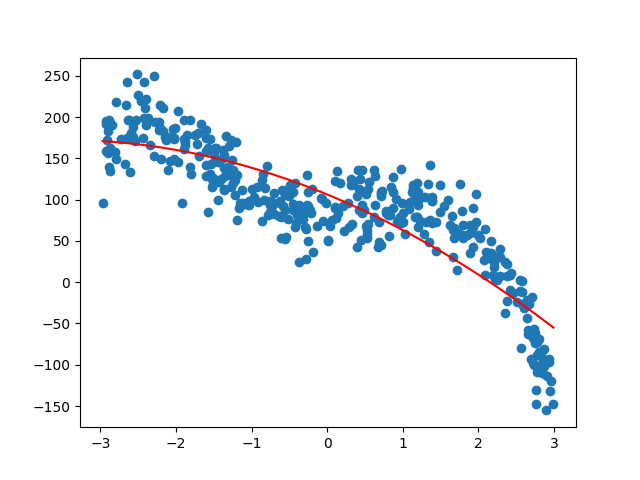
\includegraphics[width=0.5\textwidth]{../q3/degree_2.png}
    \caption{Degree 2 - underfitting}
    \label{fig:q3_1}
\end{figure}
I got severe overfitting at degree 20 and visible overfitiing at degree 18. On a k-fold cross-validation test, degree 20 had an $SS_R$ almost 1000 greater than that of degree 5 (24631 vs 23135), and at degree 25 the SSR was more than 300 times the optimal value (8681858 vs 23135).
\begin{figure}[H]
    \centering
    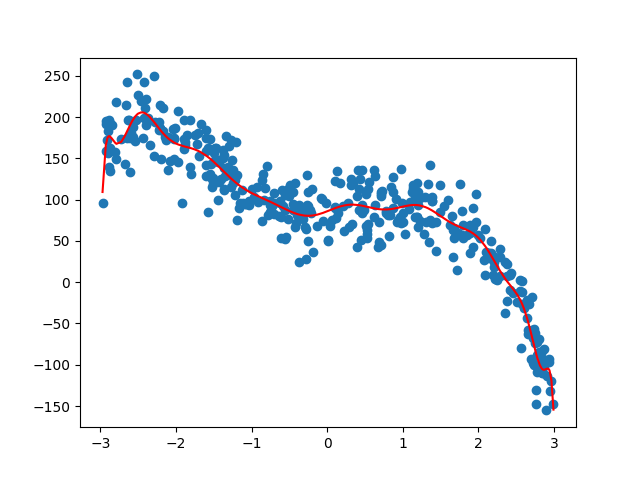
\includegraphics[width=0.5\textwidth]{../q3/degree_20.png}
    \caption{Degree 20 - overfitting}
    \label{fig:q3_2}
\end{figure}  
Optimal fitting that minimized the $SS_R$ during k-fold cross-validation with k=10 occured at degree 5. The $SS_R$ here was 23135.
\begin{figure}[H]
    \centering
    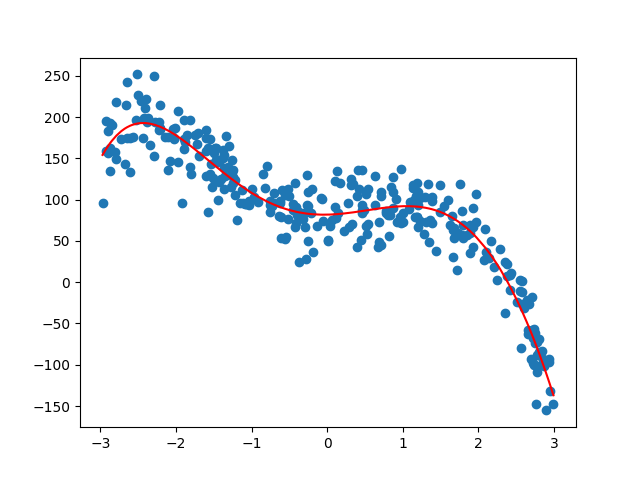
\includegraphics[width=0.5\textwidth]{../q3/degree_5.png}
    \caption{Degree 5 - optimal fitting}
    \label{fig:q3_3}
\end{figure}
\subsection{$SS_R$ and $R^2$ scores: }
The $SS_R$ scores given below are calculated as the mean of the sum of squares of residuals for roughy 10 different splits of the shuffled data on a 90-10 train-test split. The $R^2$ scores are also the average of the $R^2$ scores for the same splits.\\
The $SS_R$ scores are as follows (from degree 1 to degree 24):
[64653.555302618384, 56427.175480097954, 39251.2107718163, 24080.14499184062, 23135.01264391381, 23147.39205431092, 23316.53520429746, 23507.28378862272, 23391.932968519566, 23591.837720512074, 23799.29808194501, 24306.126217608657, 24567.738597261134, 24511.039529749152, 25040.059015164665, 24245.658838890413, 24135.381150518013, 23388.984818572288, 24449.065706832644, 24631.227983779838, 24937.833575556066, 28290.30555397866, 2673741.993952508, 12928066.182318613]\\
The scores corresponding to degree 2, degree 20 and degree 5 are 56427.175480097954, 24631.227983779838 and 23135.01264391381 respectively.\\

Similarly, the $R^2$ scores are as follows (from degree 1 to degree 24):
[0.7073677200099657, 0.7405248627800795, 0.8110940468157531, 0.885533449535035, 0.8890032715554141, 0.8890277101115677, 0.888332487004736, 0.887539875919861, 0.8879689135086817, 0.8869996684551753, 0.8860458564815987, 0.8838815115222338, 0.882803391131459, 0.8827889386885583, 0.8805258162942892, 0.8837670082600091, 0.8842901613457899, 0.8871751805158606, 0.8819040050828425, 0.8816272586091627, 0.8799340747233307, 0.8634185203165906, -17.509161117014038, -62.03234099389781]\\
The scores corresponding to degree 2, degree 20 and degree 5 are 0.7405248627800795, 0.8816272586091627 and 0.8890032715554141 respectively.\\
\newpage 